\documentclass{beamer}
\usetheme{default}
\begin{document}

\title{The Role of Light Refraction in Passive Remote Sensing}
\author{Rubén Hernández O'kelly}
\date{\today}

\begin{frame}
  \titlepage
\end{frame}

\begin{frame}{Introduction}
  \frametitle{Introduction}
  \begin{itemize}
    \item Passive remote sensing captures energy from natural sources for analysis.
    \item It provides valuable data for various fields.
  \end{itemize}
\end{frame}

\begin{frame}{The Nature of Light}
  \begin{itemize}
    \item Light as electromagnetic waves.
    \item Refraction: Change in direction when passing through different media.
  \end{itemize}

  \begin{figure}
    \centering
      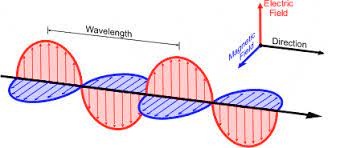
\includegraphics[width=6cm]{LightWave.jpeg}
      \caption{Light as a wave}
      \label{fig:Light}
    \centering
  \end{figure}
\end{frame}

\begin{frame}{Impact of Refraction}
  \begin{itemize}
    \item Multiple refractions in Earth's atmosphere distort light paths.
    \item Consequences for remote sensing accuracy.
  \end{itemize}
\end{frame}

\begin{frame}{Atmospheric Refraction}
  \begin{itemize}
    \item Objects displaced near horizon due to atmospheric refraction.
    \item Pronounced during sunrise and sunset.
  \end{itemize}
  \begin{figure}
    \centering
      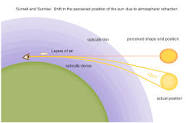
\includegraphics[width=6cm]{atm_refraction.jpeg}
      \caption{Refraction during Sunset}
      \label{fig:Light}
    \centering
  \end{figure}
\end{frame}

\begin{frame}{Water Bodies and Refraction}
  \begin{itemize}
    \item Refraction at air-water interface affects measurements.
    \item Errors in depth determination and underwater feature mapping.
  \end{itemize}
\end{frame}

\begin{frame}{Correcting for Refraction}
  \begin{itemize}
    \item Correction techniques using algorithms and models.
    \item Compensate for refraction effects during data processing.
  \end{itemize}
  \begin{figure}
    \centering
      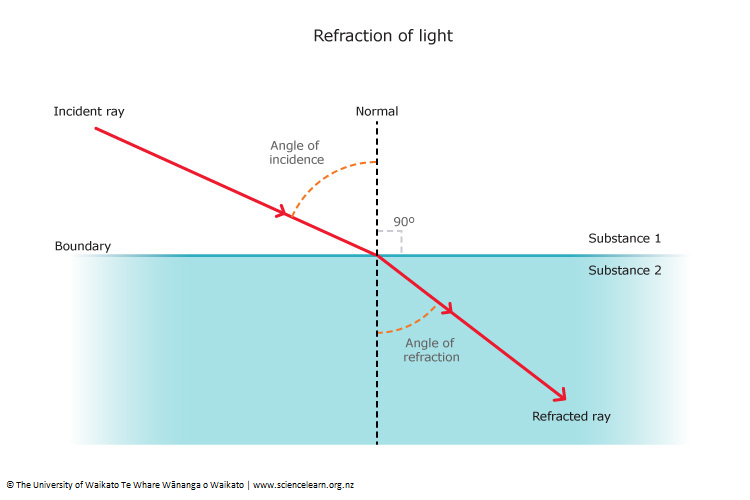
\includegraphics[width=6cm]{RefractionImage.png}
      \caption{Diagram}
      \label{fig:Light}
    \centering
  \end{figure}
\end{frame}

\begin{frame}{Conclusion}
  \frametitle{Conclusion}
  \begin{itemize}
    \item Light refraction is critical in passive remote sensing.
    \item Challenges can be overcome with correction techniques.
    \item Passive remote sensing contributes to a better world.
  \end{itemize}
  \vfill
  \centering
\end{frame}

\end{document}
